	\subsection{Taxonomy of virtualization by \textit{Bugnion}}
	
	\begin{figure}[H]
		\centering
		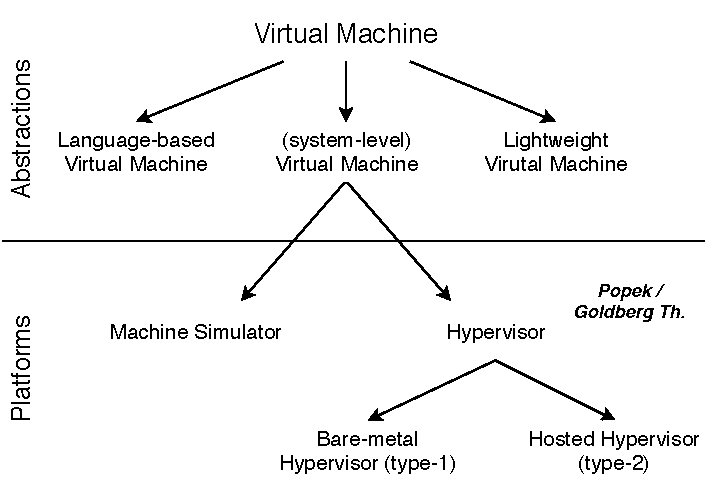
\includegraphics[width=8.5cm]{images/Bugnion2017.pdf}
		\vspace{-0.2cm}
		\caption{Basic classification of virtual machines and the platforms that run them by \textit{Edouard Bugnion, Jason Nieh, Dan Tsafrir and Margaret Martonosi} in 2017 \cite{Bugnion2017}.}
		\label{fig:TaxonomyOfVirtualizationBugnion}
	\end{figure}
	   
    In the \textit{Bugnion et al.}'s book \cite{Bugnion2017}  presents an interesting structure with two level that show the concepts related with the VMs. The first level is related with \textit{Abstraction} and its include the categories \textit{Language-base VM}, \textit{System-level VM}, and \textit{Lightweight VM}. The second level is related with \textit{Platform} and its include two categories derivative from \textit{System-level VM} called \textit{Machine Simulator}, and \textit{Hypervisor}. The latter, is divided in \textit{Bare-metal Hypervisor} also called \textit{Type-1}, and \textit{Hosted Hypervisor} also called \textit{Type-2}.
    
    \textbf{Language-based VMs} refers to the run-time environment of any managed language such as the Java Virtual Machine, Microsoft Common Language Runtime, and Javascript engines embedded in browsers.  
    
    \textbf{Lightweight VMs} refers to software mechanisms to ensure that applications run directly on the processor as securely isolated from other environments and the underlying OS. This includes examples such as Denali \cite {Whitaker2002}, Google Native Client \cite{Yee2009}, Vx32 \cite{Ford2008}, Docker \cite{Docker} y FreeBSD Jail \cite{Kamp2000}.
    
    \textbf{System-level VMs} refers to the computer environment resembles the hardware of a computer so that the VM can run an OS and its applications, in full isolation from the other virtual machines and the rest of the environment.  This category includes two types (type-1 and type2) of Hypervisor but they were already described before in this document.
    
    \textit{Bugnion et al.} is less a taxonomy than a book focusing on the core architectural support that must be provided by hardware to efficiently run virtual machines.
%	Although in the \textit{Bugnion et al.}'s study \cite{Bugnion2017} there is an interesting way to classified VMs when presenting Platform / Abstractions separation. However, the level of detail presented is superficial and leaves out of consideration many other elements that are part of virtualization technologies.
	
	